%%%%%%%%%%%%%%%%%%%%%%%%%%%%%%%%%%%%%%%%%%%%%%%%%%%%%%%%%%%%%%%%%%%%%%%%%
%Objetivo: 
%Autor:
%Data Criação:
%Data Modificação:
%Data Revisão:
%%%%%%%%%%%%%%%%%%%%%%%%%%%%%%%%%%%%%%%%%%%%%%%%%%%%%%%%%%%%%%%%%%%%%%%%%%
\chapter{Pesquisa com Profissionais}
\label{ch:pesquisa-profissionais}

\section{Introdução}
\label{sec:pesquisa-profissionais-intro}

Uma pesquisa baseada em questionários, conhecido na literatura como
\textit{Survey}, é uma abordagem de coleta e análise de dados na qual os
participantes respondem a perguntas ou declarações que foram desenvolvidas
antecipadamente~\cite{kasunic2005designing}. Este tipo de pesquisa
dividem-se em duas grandes categorias: questionários auto-administrados e
entrevistas~\cite{kasunic2005designing}. O primeiro tipo é aquele que a a
maioria das pessoas pensa quando falamos em  ``pesquisa de opinião'', no qual
geralmente recebemos por meio de correio eletrônico ou estão disponíveis através
de páginas da Internet. As entrevistas apresentam as mesmas característica dos
questionários auto-administrados, estando a principal diferença na profundidade
que as perguntas são apresentadas aos participantes.  Neste estudo utilizamos
um questionário auto-administrado como instrumento de coleta dos dados.

Em uma pesquisa baseada em questionário os participantes responder a perguntas
ou afirmações que foram que foram desenvolvidas com antecedência. Quando
conduzida adequadamente, esse tipo de pesquisa permite que os pesquisadores
generalizem as crenças e opiniões de uma população mediante os dados
coletados de um subconjunto do público-alvo (amostra). No trabalho conduzido por
Kasunic~\cite{kasunic2005designing} são apresentada um conjunto de etapas a
serem seguidas no processo de condução de um survey:

\begin{enumerate}
\item{Identificar os objetivos da pesquisa}
\item{Identificar e caracterizar o público-alvo}
\item{Elaborar o plano de amostragem}
\item{Elaborar e escrever um questionário}
\item{Aplicar questionário de teste ou piloto}
\item{Distribuir o questionário}
\item{Analisar os resultados e escrever o relatório}
\end{enumerate}

Em uma série de artigos~\cite{pfleeger2001principles,pfleeger2002principles},
Kitchenham e Pfleeger discutem os princípios da pesquisa com questionário no
âmbito da Engenharia de Software (ES), tendo como foco principal as etapas 3, 4,
6 e 7 descritas no estudos feito por Kasunic~\cite{kasunic2005designing}. Os
autores apresentam conceitos básicos de estatística para discutir algumas
questões relativas à população e amostra. Nestes mesmos estudos os autores
investigaram o desenho de quatro surveys na área de ES e concluem que em
apenas um deles foi composto por uma amostra significativa de uma população. Ao
final eles salientam a necessidade que este tipo estudo científico utilize uma
metodologia de modo a reduzir qualquer viés no tocante à amostra utilizada.

Com o objetivo de coletar os aspectos mais importantes das funcionalidades
oferecidas pelas Ferramentas de Gerenciamento de Requisições de Mudança (FGRM)
do ponto de vista dos profissionais ligados à manutenção de software foi
realizada uma pesquisa com profissionais (survey). O planejamento e o desenho da
pesquisa seguiu as diretrizes propostas nos trabalhos de
Wohlin~\cite{wohlin2012experimentation} e Kasunic~\cite{kasunic2005designing}.
Em especial, no tocante a definição da população e da amostra de interesse
utilizamos o arcabouço (framework) proposto por De Mello e
outros~\cite{de2015investigating, de2014towards}.

A população da pesquisa proposta é a comunidade envolvida com o processo de
manutenção de software e que faça uso de FGRM's. Desta utilizamos  como amostra
os profissionais que estão envolvidos nos projetos
Python\footnote{\url{http://bugs.python.org/}}, Eclipse
Foundation\footnote{\url{https://bugs.eclipse.org/bugs/}}, Mantis Bug
Tracker\footnote{\url{https://mantisbt.org/}} que contemplam os profissionais
vinculados a algum projeto de código aberto. Por outro lado, visando alcançar os
profissionais que trabalham em empresas privadas, utilizamos profissionais que
fazem parte das rede sociais Stack Oveflow e LinkedIn e que façam parte de
discussões na rede de assuntos relacionados à manutenção de software. A pesquisa
foi replicada em uma empresa pública de software do qual o autor possui vínculo.
Maiores detalhes sobre o processo de escolha das amostras serão discutidas
posteriormente.

A importância deste tipo de trabalho está na possibilidade de avaliar se as
pesquisas relativas a evolução das funcionalidades das FGRM's estão em
consonância com as necessidades dos profissionais envolvidos em manutenção de
software, reduzindo, desta forma, a distância entre o estado da arte e o estado
da prática.

\section{Objetivo da Pesquisa com Profissionais}
\label{sec:objetivo_da_pesquisa_com_profissionais}
Em linhas gerais, o objetivo desta etapa do estudo é analisar, através da
percepção e opinião dos profissionais envolvidos em manutenção de software, a
situação das funcionalidades atualmente oferecidas pelas FGRM's, bem como
a adotação das metodologias propostos pelos agilistas no processo de manutenção
de software.

Para uma melhor apresentar a finalidade desta parte da dissertação estruturamos
o objetivo conforme propõe a metodologia GQM (Goal, Question e
Metric)\cite{gqm}, \textit{o propósito deste estudo avaliar as funcionalidade
	oferecidas e as extensões propostas nas literatura ponto de
	vista dos profissionais envolvidos em manutenção de software no contexto de
	projetos de software de código aberto e uma empresas privadas e  uma empresa  pública informática de
	médio porte.}

Com intuito de atingir os objetivos propostos fora definidas as seguintes
questões de pesquisa:
\todo[inline]{Incluir uma descrição para cada questão de
	pesquisas}
\begin{description}
	\item[Questão 01] Qual a opinião dos profissionais envolvidos em Manutenção
		de Software com relação as funcionalidades oferecidas atualmente pelas
		FGRM\@?
	\item[Questão 02] Na visão  dos profissionais envolvidos em Manutenção de
		Software quais das extensões propostas na literatura teriam maior
		relevância em suas atividades atuais?
	\item[Questão 03] Como as práticas propostas pelos agilistas estão sendo
	utilizadas especialmente no processo de manutenção de software?
	\item[Questão 04] Como as FGRM's podem ajudar aos times devotados à manutenção
	de software na prática adotada pelos agilistas?
\end{description}

As questões de pesquisas foram respondidas mediante a realização de uma pesquisa
baseada em questionário (survey). O desenho da pesquisa é detalhada na próxima
seção onde discutimos a estrutura do questionário bem como a amostra a população
e a sua respectiva amostra utilizada no estudo.

\section{Desenho e Metodologia da Pesquisa com Profissionais}
\label{sec:desenho_da_pesquisa_com_profissionais}

\subsection{Conceitos Básicos}
Estudos primários em Engenharia de Software (SE) são muitas vezes conduzidos em
amostras estabelecidas por conveniência (Pickard et al., 1998, Sjøberg et al.,
2005, Dybå et al., 2007). Este cenário é especialmente crítico para os
levantamentos em grande escala (Kasunic 2005), nos quais são aplicados esforços
consideráveis no recrutamento e recolha de dados dos participantes (Conradi et
al., 2005), mas a generalização dos resultados é limitada, mesmo quando as
características de outros inquéritos são claramente descritas e Repetidos em
seus ensaios.

Um desafio no estabelecimento de amostras representativas nos inquéritos SE
inclui a identificação de fontes relevantes e disponíveis a partir das quais
podem ser estabelecidas estruturas de amostragem. Portanto, os pesquisadores da
SE são tentados a explorar fontes alternativas tipicamente disponíveis na Web
para ampliar o tamanho das amostras, como as redes sociais (de Mello e
Travassos, 2013). No entanto, o uso ad hoc dessas tecnologias Web por si só não
é suficiente para evoluir o cenário de amostragem em relação aos levantamentos
SE, uma vez que o tamanho das amostras é apenas uma das questões que dificultam
a generalização dos resultados das pesquisas SE

Esta Pesquisa com Profissionais (survey) consistiu de um estudo exploratório sem
uma hipótese prévia a ser avaliada. Realizamos um survey com um desenho
trans-seccional\cite{kitchenham2002principles} onde a nossa população de
interesse são os profissionais envolvidos em manutenção de software e estamos
especialmente interessado na experiência deles no uso das FGRM\@.

Conforme discutido anteriormente, a população de interesse desta pesquisa é
composta por profissionais envolvidos em desenvolvimento e manutenção de
software. Para sistematizar o processo de escolha da amostragem utilizamos o
arcabouço (framework) conceitual proposto por de Mello e
outros~\cite{de2014towards} que está representado na
Figura~\ref{fig:framework-amostragem}. O modelo proposto inclui além dos
conceitos estatísticos tradicionalmente utilizados em pesquisas por questionário
(surveys), tais como público-alvo, população, amostragem e unidade de
observação~\cite{thompson2012sampling}, introduz um conjunto de novos conceitos
que visam apoiar o processo de escolha da amostragem em questionários,
especialmente em ES\@. Os conceitos que os autores propuserem incluem:
\textit{Fonte de Amostragem, Unidade de Pesquisa, Plano de Pesquisa e Estratégia
	de Amostragem}.

\begin{figure}[htpb]
	\centering
	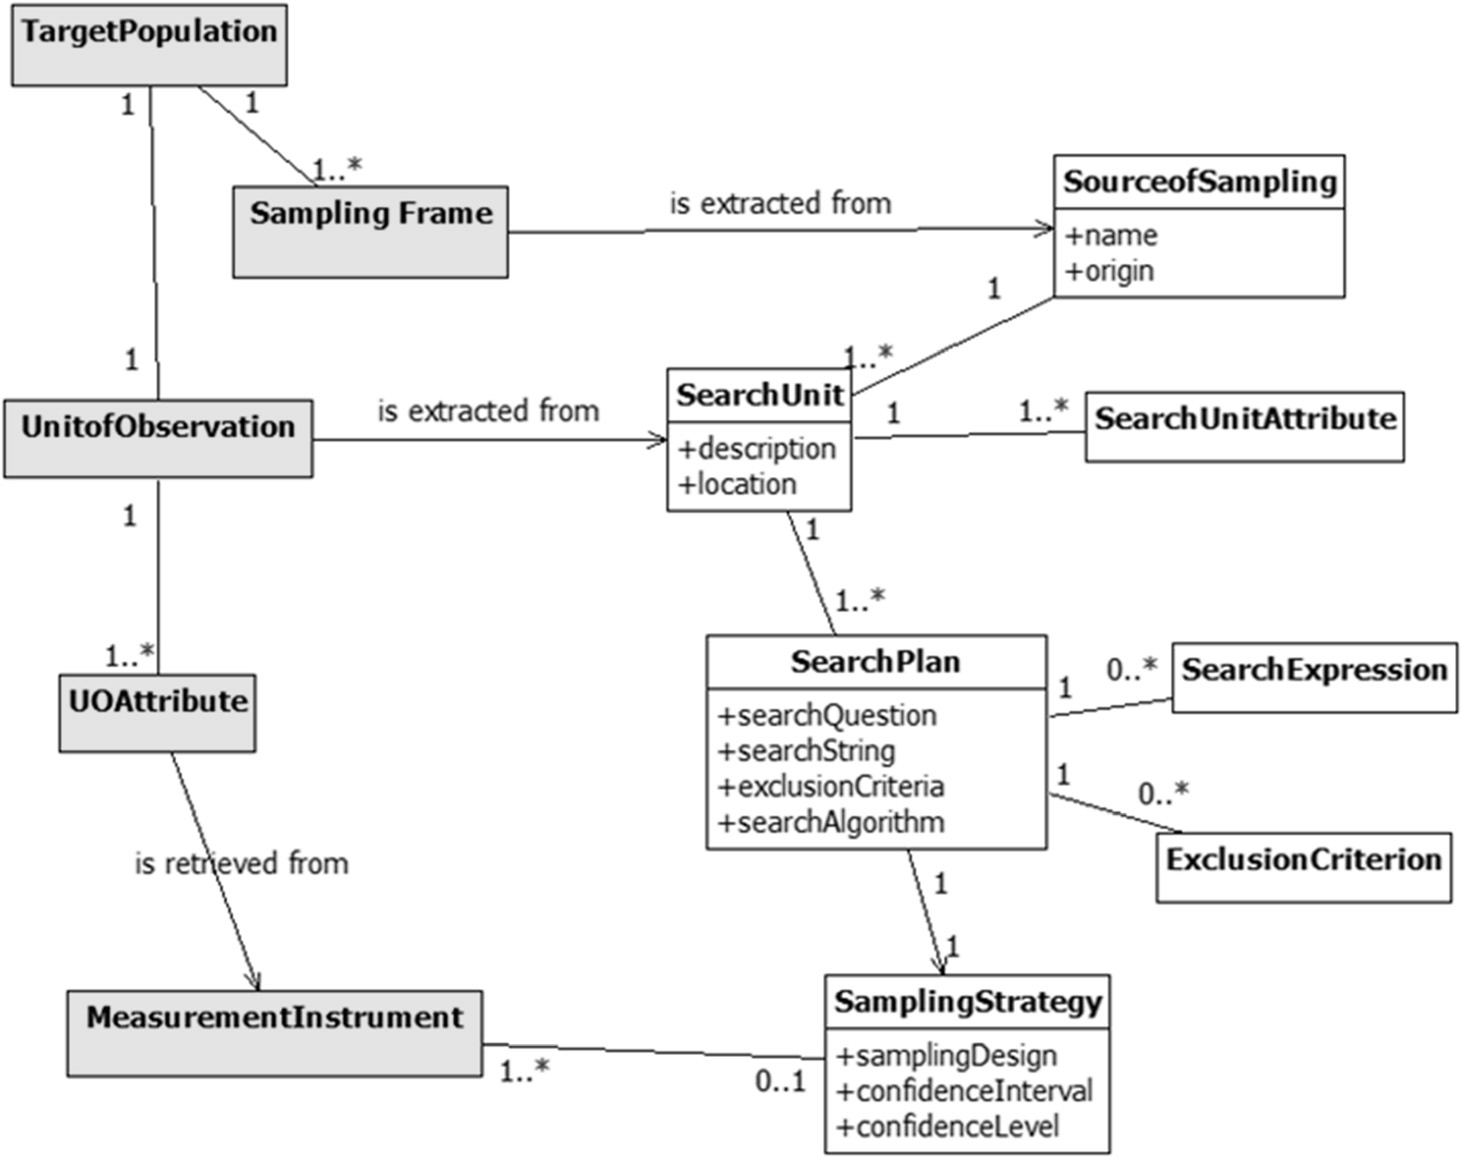
\includegraphics[width=0.8\linewidth]{./chapter-pesquisa-com-profissionais/img/framework-amostragem.png}
	\caption{Os conceitos que compõem o Arcabouço Conceitual proposto por de
		Mello. Extraído de~\cite{de2015investigating}}
\label{fig:framework-amostragem}
\end{figure}


\todo[inline]{Incluir definição de Unidade de Observação}
Uma \textit{Unidade de Observação}~\cite{wohlin2012experimentation}

Uma \textit{Unidade de Pesquisa} caracteriza como uma ou mais \textit{Unidade de
	Observação} podem ser recuperadas de uma \textit{Fonte de Amostragem}
específica. O \textit{Plano de Pesquisa} descreve como \textit{Unidades de
	Pesquisa} serão sistematicamente recuperadas de uma Fonte de Amostragem e
avaliadas para compor a amostragem da pesquisa. Finalmente, a Estratégia de
Amostragem descreve as etapas que devem ser seguidas para definição da
amostragem e recrutamento de indivíduos que participarão do estudo.

Uma \textit{Fonte de Amostragem} consiste de um banco de dados, que não
necessariamente é automatizado, em que um subconjunto válido do público-alvo
pode ser sistematicamente recuperado, além de permitir a extração aleatória de
amostra da população de interesse. Sendo assim, os autores afirmam que no caso
de determinada Fonte de Amostragem ser considerada válida para um contexto de
pesquisa específico, pode-se concluir que as amostras podem ser extraídas desta
fonte a fim de serem utilizados no mesmo contexto de pesquisa. Para ser
considerada válida, uma Fonte de Amostragem deve satisfazer, pelo menos, os
seguintes Requisitos Essenciais (Essential Requirements\@-\@ ER):

\begin{description}
	\item[ER1] Uma Fonte de Amostragem não deve representar intencionalmente um
		subconjunto segregado do público-alvo, ou seja, dado um público-alvo
		\textit{``X''}, não seria adequado pesquisar por unidades da fonte
		intencionalmente desenhada para compor um subconjunto específico de
		\textit{``X''}.
	\item[ER2] Uma Fonte de Amostragem não deve apresentar qualquer viés em
		incluir na sua base de dados determinados subconjuntos do público-alvo.
		Critérios desiguais para inclusão de Unidades de Pesquisa significam
		oportunidades desiguais para oportunidades de amostragem.
	\item[ER3] Todas as Unidades de Pesquisa das amostras e suas Unidades de
		Observação devem identificados por de forma única.
	\item[ER4] Todas as amostragem de determinada Unidade de Pesquisa devem ser
		acessíveis. Se houver unidades de pesquisa ocultas, não é possível
		contextualizar a população.
\end{description}

Os autores outros requisitos que são definidos como desejáveis que estão
relacionados com amostragem, clareza e integridade da amostra. Os critérios
adicionais e exemplos de avaliação de Fontes de Amostragem utilizados os
requisitos discutidos podem ser encontrado no estudo proposto por de Mello e
outros~\cite{de2014towards}.

\subsection{Metodologia}

No caso desta pesquisa, o público-alvo é composto por profissionais devotados em
desenvolvimento e manutenção de software. O perfil do participante da população
de interesse é bastante geral, uma vez que um conjunto de características e
práticas deste tipo de profissional é bastante diversa e pode depender de
questões como processo de software utilizado, linguagem de programação
utilizada, tipo de projeto no qual está envolvido, dentre outras. Assim, todos
os profissionais que trabalham em projetos de software, sejam estes projetos de
código aberto ou de empresas privadas, podem potencialmente contribuir com esta
investigação. É importante destacar que cabe ao Plano de Pesquisa avaliar quando
a relevância do participante utilizando, por exemplo, o nível de experiência do
respondente como critério de inclusão. As subseções a seguir descrevem a
estratégia de recrutamento projetada para a pesquisa com profissionais
realizada neste estudo.

\subsubsection{Fonte de Amostragem, Unidade de Pesquisa e População}

Para a realização deste estudo foi estabelecida 05 diferentes Fontes de
Amostragem conforme exibido na Tabela~\ref{tab:fontes-amostragens}. Estas fontes
foram selecionadas de modo a incluir profissionais que estão se dedicam a
projetos de código aberto (Python, Eclipse, MantisBT) e aqueles que
possivelmente façam parte de empresas privadas de desenvolvimento e manutenção
de software. Para o primeiro grupo, escolhemos projetos de código aberto que
tivessem pelo menos 5 anos de existência, possuem uma comunidade bem
estabelecida e permitam acesso aos dados de suas FGRM's. Além disso, escolhemos
projetos que utilizem diferentes FGRM's como o objetivo de abarcar diferentes
experiências de uso deste tipo de ferramenta. Para alcançarmos os profissionais
que trabalham em empresas privadas de desenvolvimento de software utilizamos  as
redes sociais LinkedIn e Stack Overflow. Tais redes foram selecionas
especialmente por conta de sua cobertura, que contam com e um mais de 6 milhões
de usuários para o caso do Stack
Overflow~\footnote{\url{http://stackexchange.com/sites}} e mais de 10 milhões de
profissionais de TI espalhados pelo mundo, quando falamos do
LinkeIn~\cite{de2014towards}.

\begin{table}[htb]
\centering
\resizebox{\textwidth}{!}{%
\begin{tabular}{|llc|}
\hline
\multicolumn{1}{|c}{\textbf{Fonte de Amostragem}} & \multicolumn{1}{c}{\textbf{URL}}                & \textbf{Membros} \\ \hline
Python                                            & https://bugs.python.org/                        & $\sim$19 K       \\
Eclipse Foundation                                & https://bugs.eclipse.org/bugs/                  & $\sim$2.6 K      \\
MantisBT                                          & http://www.mantisbt.org/bugs/my\_view\_page.php & $\sim$40 K       \\
LinkeIn                                           & https://www.linkedin.com/                       & $\sim$347 M      \\
Stack Overflow                                    & http://stackoverflow.com/                       & $\sim$6.6 M      \\ \hline
\end{tabular}%
}
\caption{Fontes de Amostragem utilizadas no estudo.}
\label{tb:fonte-de-amostragens}
\end{table}

No escopo deste estudo a lista de Requisições de Mudanças no projetos de código
aberto serão a Unidade de Pesquisa a ser considerada. Desde que o LinkedIn
permite realizar pesquisa abrangente de ``grupo de interesse'', serão estes as
Unidades de Pesquisa. No caso da rede social Stack Overflow foi considerada cada
discussão proposta por um usuário (thread) foi considerada como a Unidade de
Pesquisa. Em todas as Fontes de Amostragem foram coletados os seguintes
atributos: Nome do Participante, E-mail do Participante, Data de Interação e
Tipo de Interação. No caso do LinkedIn utilizamos um métrica
adicional da própria rede social conhecida como
reputação~\footnote{\url{http://stackoverflow.com/help/whats-reputation}} que é
uma medida aproximada de quanto a comunidade poderia confiar em você. A medida é
calculada quando o usuário com base nas ações do usuário e em como a comunidade
avalia tais ações. Neste trabalho a métrica foi utilizada para verificar a
frequência de participação de determinado usuário em discussões sobre manutenção
ou desenvolvimento de software. Em resumo, podemos considerar que as pessoas que
fazem parte dos projetos de código aberto, os participantes de grupo de
interesse do LinkeIn e das discussões do Stack Overflow  que compõe a população
a ser considerada neste estudo.

\subsubsection{Unidade de Observação e Unidade de Análise}

Nesta pesquisa, a Unidade de Observação e a Unidade de Análise são a mesma
entidade (indivíduo) e cada membro distinto de cada grupo é potencialmente
considerado uma unidade válida a ser amostrada. Os seguintes atributos devem ser
coletados de cada um:
\begin{itemize}
	\item Nome do Participante
	\item E-mail do Participante
	\item Data de Interação
	\item Tipo de Interação
\end{itemize}

O Tipo de Interação representa a ação que o participante realizou na Fonte de
Amostragem, por exemplo relatar uma RM, finalizar uma RM, responder a uma
pergunta e etc. Estes atributos foram utilizados para avaliar se determinada
Unidade de Observação (indivíduo) será incluído na Fonte de Amostragem. Outros
atributos foram coletados através do questionário de pesquisa (instrumento de
medição): localização geográfica, tempo de experiência, nome da função
desempenhada, principais atribuições, dentre outros.

\subsubsection{Plano de Pesquisa}

De modo a construir as Unidade de Pesquisa que foram utilizadas neste estudo,
utilizamos três estratégias distintas cada uma relacionada as características da
Fonte de Amostragem utilizada. Para as fontes que foram coletadas de projetos de
código aberto (Python, Eclipse e MantisBT) utilizamos os registros históricos
das RM's ocorridos nos últimos 05 anos. Além disso registro a frequência com o
qual um participante teve contato com o projeto. Esta última métrica nos
permitiu selecionar os participantes que tenham um mínimo de interação com
projeto.

No caso do LinkedIn realizamos a busca por grupos de interesse utilizando as
sentenças de busca descritas na Figura~\ref{fig:setencas-grupos}. Um conjunto
similar de sentenças de busca foi utilizado no mapeamento sistemático  descrito
no Capítulo~\ref{ch:mapeamento-sistematico}.

\begin{figure}[htpb]
	\centering
	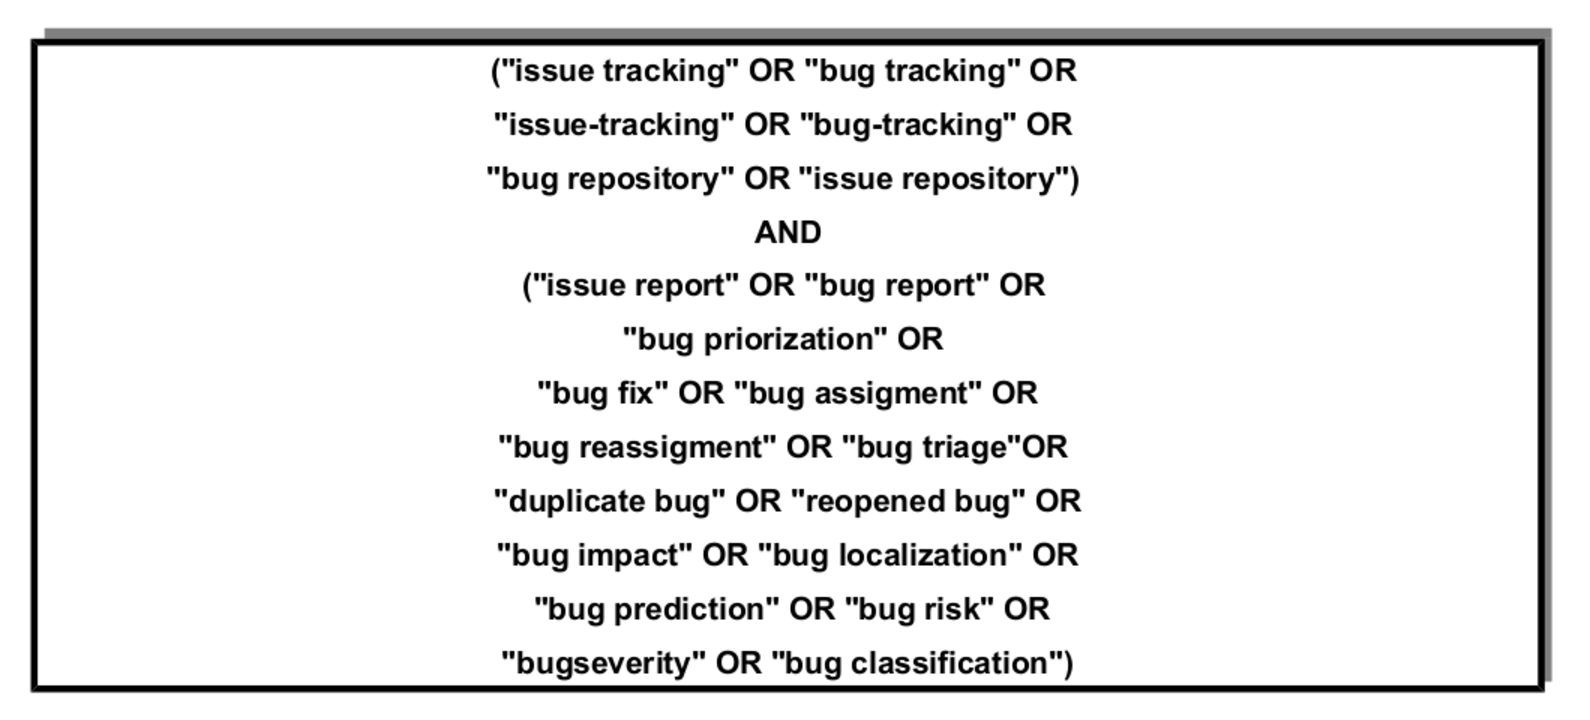
\includegraphics[width=0.8\linewidth]{./chapter-pesquisa-com-profissionais/img/setencas-grupos.pdf}
	\caption{Sentenças utilizadas para escolhas dos grupos do LinkedIn e de
		discussões no Stack Overflow}
\label{fig:setencas-grupos}
\end{figure}

Para a rede social Stack Overflow utilizamo a busca oferecida pelo próprio
site~\footnote{\url{http://data.stackexchange.com/}} de modo a encontrar
discussões que se encaixam com as sentenças apresentas na
Figura~\ref{fig:setencas-grupos}. Neste contexto, visando restringir a seleção
de grupos de participantes que estejam vinculados à desenvolvimento e manutenção
de software realizamos a exclusão dos dados de participantes que:

\begin{itemize}
	\item Proíbem expressamente a utilização dos seus dados, especialmente do
		seu endereço eletrônico, para a realização de estudos;
	\item A Fonte de Amostragem ao qual pertence não possui um mínimo de 05 anos
		de registros
	\item Para os grupos do LinkedIn e Stack Overflow, aqueles que restringem
		explicitamente a mensagem individual entre seus membros;
    \item Utilizam uma língua diferente do inglês, tendo em vista que o idioma
		inglês é padrão em fóruns internacionais e apenas existiam uma versão em
		inglês e português para o questionário utilizados.
\end{itemize}

\subsubsection{Estratégia de amostragem}

Apesar das Fontes de Amostragens terem sidos extraídos de diferente locais, pode
ocorrer que uma sobreposição de participantes, ou seja, um mesmo participante
estar em duas ou mais fontes. Para minimizar a possibilidade da duplicação de
participação de uma mesma unidade de observação realizamos uma  desenho de
amostragem conhecido como Agrupada. Uma Amostragem agrupada pode ser aplicada
quando grupos homogêneos (clusters) compostos por unidades distintas podem ser
identificados numa população. Como consequência, devido a essa similaridade,
apenas um subconjunto desta população pode ser utilizada como amostra de forma
aleatória aleatoriamente sem perda significativa de
confiança~\cite{thompson2012sampling}. Assim, a amostragem em  agrupamentos é
comumente aplicada em pesquisas em larga escala nas quais os pesquisadores têm
restrições operacionais para recrutar e coletar
dados~\cite{roberts2004mortality}.

\subsubsection{Extração de Dados}

Para extrair os atributos necessários de cada participante desta pesquisa
utilizamos três estratégias distintas. No caso da rede social Stack Overflow
utilizamos uma ferramenta da web oficial que permite compartilhar, consultar e
analisar os dados de todos os sites da rede Stack
Exchange~\footnote{\url{http://data.stackexchange.com/stackoverflow}}. A
ferramenta possibilita a utilização da linguagem SQL para acesso aos dados e
apresenta o respectivo modelo de dados para facilitar a consulta. A
Figura~\cite{fig:stack-exchange}. A ferramenta permite a extração no formato CSV
(Comma Separated Values) o qual foi inserido em um banco de dados para posterior
aplicação das regras de inclusão e exclusão.

\begin{figure}[htpb]
	\centering
	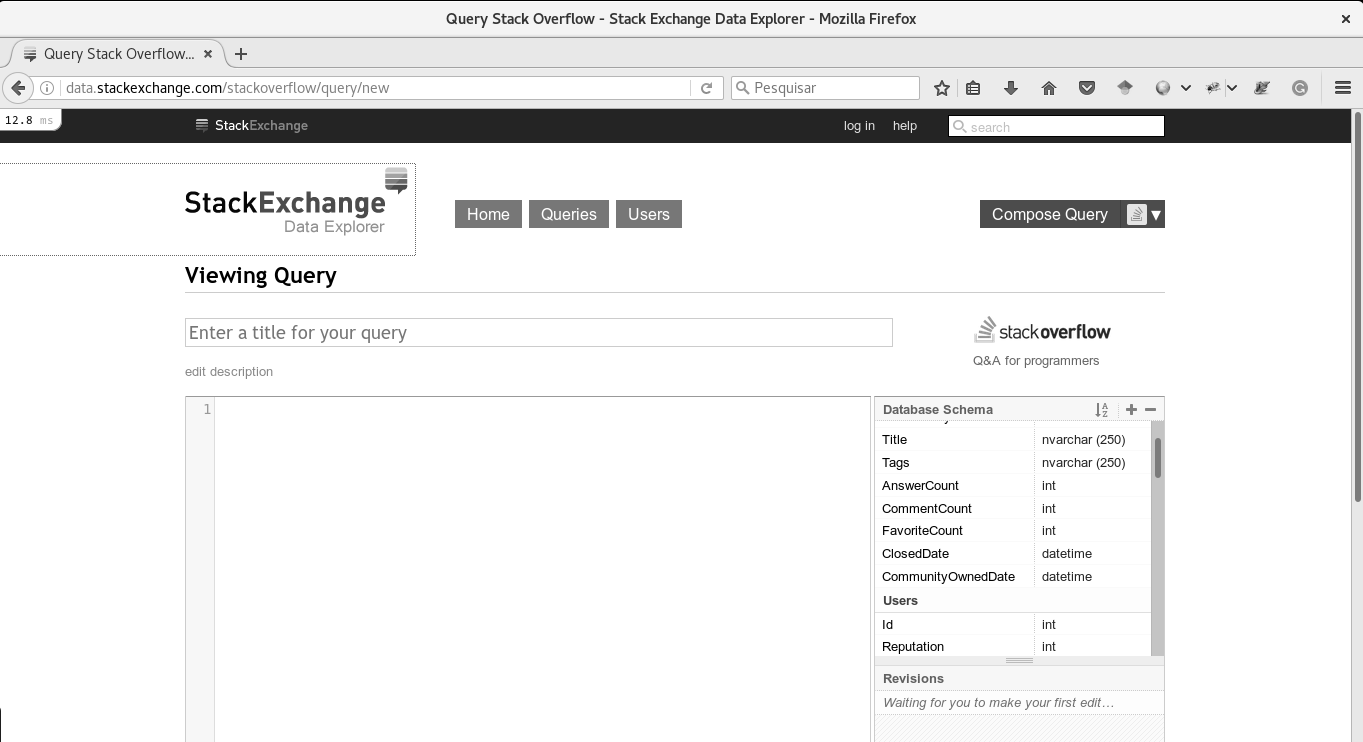
\includegraphics[width=0.8\linewidth]{./chapter-pesquisa-com-profissionais/img/stack-exchange.png}
	\caption{Ferramenta de coleta de dados da rede Stack Overflow}
\label{fig:stack-exchange}
\end{figure}

Para os projetos de código aberto (Python, Eclipse e MantisBT) foi desenvolvido
um Web Crawler para coletar as informações dos participantes. Um Web Crawler
(rastreador web) é um programa de computador que navega pela World Wide Web de
uma forma metódica e automatizada. A partir de uma lista de Requisições de
Mudança previamente coletadas a ferramenta coleta os dados dos participantes a
partir do histórico de modificações de determinada RM\@. A
Figura~\cite{fig:historico-rm-python} apresenta o histórico de registros de uma
RM do projeto Python onde os dados dos participantes podem ser visualizados nos
quadros inseridos. A ferramenta utiliza uma marca HTML <a> e seu valor de
classe (título, ou seja, nome de membro) para coletar os dados. De modo similar
ao que foi realizados com os dados do Stack Overflow as informações extraídas
foram armazenadas em um banco de dados para posterior aplicação de critérios de
inclusão.

\begin{figure}[htpb]
	\centering
	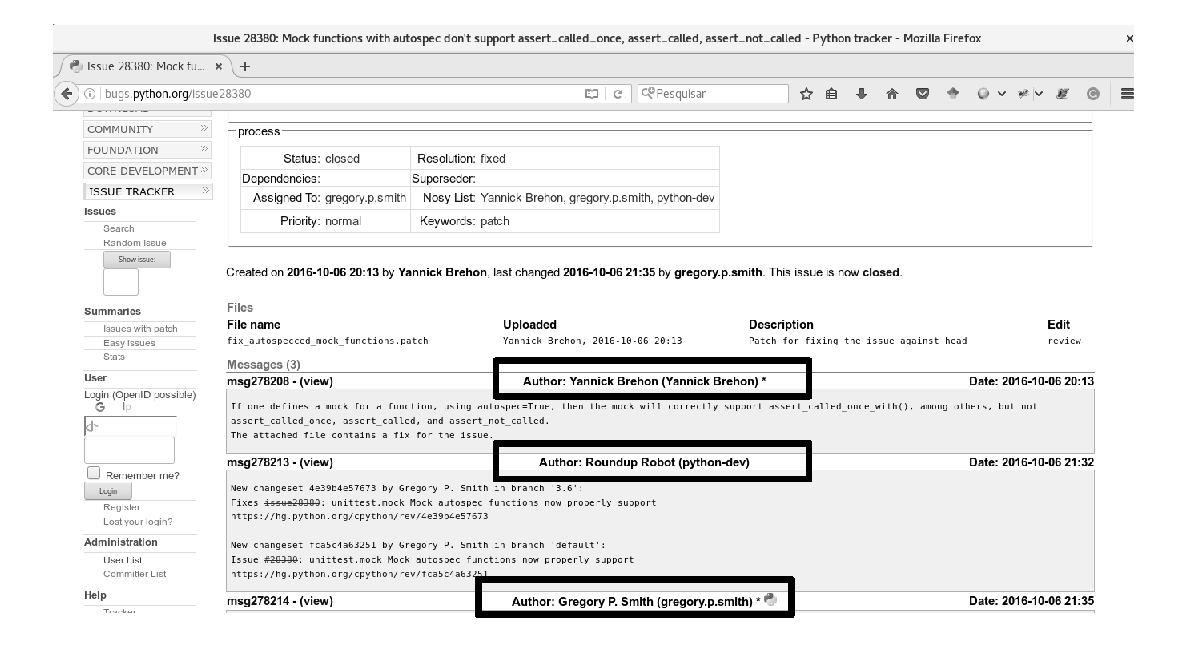
\includegraphics[width=0.8\linewidth]{./chapter-pesquisa-com-profissionais/img/historico-rm-python.pdf}
	\caption{Histórico de relatos de uma RM do projeto Python}
\label{fig:historico-rm-python}
\end{figure}

No caso da Fonte de Amostragem do LinkedIn utilizamos a busca já existente na
ferramenta utilizando as sentenças de busca exibidas na
Figura~\ref{fig:setencas-grupos}. Para extrair os atributos necessários de cada
foi utilizada uma extensão do Firefox chamada
iMacros~\footnote{\url{http://imacros.net/}}.  Este plugin torna possível
selecionar valores de tags HTML e salvá-los como arquivo CSV (Comma Separated
Values). Além disso ele permite o envio de mensagem aos membros de forma
automatizada.

Os dados coletados nas diferentes Fontes de Amostragem foi inicialmente
extraídos e salvos no formato CSV\@. Todavia, o arquivo CSV contém muitos dados
indesejados e artefatos de texto que devem ser removidos. Neste caso, foi
necessário a realização de um processo de limpeza e transformação das informação
antes do envio propriamente dito aos participantes.

\subsubsection{Questionário}
\label{subsec:questionario}

O formulário enviado aos participantes foi estruturado em três parte, cada uma
com o objetivo de coletar um conjunto de informações. Na primeira parte estamos
interessados na formação de base (background) dos profissionais. O segundo
conjunto de perguntas visa obter a percepção dos participantes sobre as
funcionalidades atualmente oferecidas pelas FGRM\@. A terceira parte é do
formulário contêm as perguntas sobre a percepção dos participantes sobre as
extensões propostas na literatura.

A fim de obtermos um formulário que conseguisse atingir os objetivos deste
estudo, realizamos um processo de avaliação em quatro etapas. O formulário
resultante de uma etapa anterior foi utilizado como entrada de uma etapa
posterior. Desta forma, utilizamos um processo iterativo para produzirmos o
formulário.
\begin{enumerate}[(i)]
	\item Avaliação por Pesquisadores: Nesta etapa o formulário inicialmente
		proposto foi enviado para dois pesquisadores experientes na área de
		manutenção de software.
	\item Avaliação por Profissionais O formulário resultante da análise
		anterior foi encaminhado a dois profissionais experientes envolvidos com
		manutenção de software.
	\item Piloto da Pesquisa O formulário obtido após a fase anterior foi
		utilizado em um piloto com
		dez profissionais envolvidos da manutenção de software de uma empresa
		pública de
		informática~-~PRODABEL\footnote{\url{{http://www.prodabel.pbh.gov.br}}}
	\item Tradução do Formulário Em cada uma das etapas de anteriores o
		formulário foi aplicado em
		português, tendo em vista que alguns profissionais envolvidos no
		processo de avaliação não
		ter fluência em língua inglesa, em especial na fase ``Piloto da
		Pesquisa'. Neste sentido, a última etapa  consistiu na tradução do
		formulário para a língua inglesa.  Esta etapa foi conduzida com  o
		suporte de um pesquisador experiente na área de Engenharia de Software.	
\end{enumerate}

\subsubsection{Envio da Mensagem}

A fim de viabilizar e mitigar os riscos operacionais do envio manual de
mensagens ao participantes foi desenvolvido um processo automatizado de envio de
mensagens ao participantes. Excetuando o caso do grupos do LinkedIn, onde a
mensagem foi enviada utilizado uma funcionalidade própria da ferramentas, o
demais participantes foram convidados mediante correio eletrônico. O processo de
envio seguiu uma política que consiste  em enviar uma mensagem ao participante
com base em um modelo. Após um um prazo de dois dias uma mensagem de lembrete.
As mensagens foram preenchidas (uma a uma) e enviadas através de correio
eletrônico para cada um dos participantes com base no seguinte modelo:

\fbox{\begin{minipage}{\textwidth}
Dear \{\{ nome do participante\}\}\!

I’m Vagner Clementino (\url{homepages.dcc.ufmg.br/~vagnercs}), Master Student at
Federal University of Minas Gerais, Brazil. I’m conducting a research,
supervised by Prof\. Rodolfo Resende \@-\@ \url{homepages.dcc.ufmg.br/~rodolfo}
concerned with improvements in Issue Tracking System. As part of them, we
planned and executed a survey aiming at to reach a large-scale population of
researchers/practitioners interested on to improve the features of the Issue
Tracking Systems. Based on your area of interest, we kindly invite you to take
part in the following survey:

\{\{url do formulario\}\}

You was chosen because your relevant participation/contribution in \{\{nome da
		fonte de amostragem\}\}\@-\@ \{\{url da fonte de amostragem\}\}. Your opinion is
essential to strength our findings. Please, help us accordingly your
possibilities by answering this survey until January 29th. As soon as we
conclude data analysis, we will share the results with all participants and the
software engineering community. If you have already fulfilled this
questionnaire, please ignore this email.

Thanks in advance,
Vagner Clementino

\end{minipage}}

\subsection{População, Amostra e Respostas}
\label{subsec:populacao_amostra_respostas}

\section{Resultados}
\label{sec:analise_dados}

Neste seção apresentamos os resultado obtidos da aplicação do questionário. Os
foram divididos pela questão de pesquisa ao qual visa responder. Por se tratar
de um estudo exploratório, no qual não foi proposta determinada tese a ser
provada, a análise dos resultados é feita mediante o uso de gráficos
representando a escala de Likert. Este tipo de grafo é recomendado para
visualizar dados na escala de Likert tendo em vista que possibilita o
entendimento da divergência entre as respostas dos
participantes~\cite{robbins2011plotting}

\subsection{Perfil dos Participantes}
\label{sub:perfil_dos_participantes}

\section{Discussão}

\section{Ameças à Validade}

\subsubsection{Ameaças Internas}
\label{ssub:Ameacas_internas}

\subsubsection{Ameaças Externas}
\label{ssub:Ameacas_externas}


\section{Resumo do Capítulo}
\label{sec:resumo_do_capitulo}
